\documentclass[tikz,border=8pt]{standalone}
% Shared look for every TikZ diagram. Load with \input{../../tools/tikz-style.tex}
\usepackage[T1]{fontenc}
\usepackage{lmodern}
\renewcommand{\sfdefault}{lmr}  % diagrams use the same serif as the text
\usetikzlibrary{arrows.meta, positioning, shapes.geometric, calc, fit, backgrounds}
\definecolor{cblue}{HTML}{4C78A8}
\definecolor{corange}{HTML}{F58518}
\definecolor{cgreen}{HTML}{54A24B}
\definecolor{cred}{HTML}{E45756}
\definecolor{cpurple}{HTML}{B279A2}
\definecolor{cgrey}{HTML}{6B6B6B}
\tikzset{
  every picture/.style={font=\sffamily, line width=1.2pt},
  box/.style={draw=#1, fill=#1!12, rounded corners=4pt, align=center, inner sep=7pt, minimum height=1.1cm},
  box/.default=cgrey,
  arrow/.style={-{Stealth[length=3mm]}, draw=cgrey, line width=1.4pt},
  title/.style={font=\sffamily\bfseries\Large},
  note/.style={font=\sffamily\small, text=cgrey, align=center},
}
\AtBeginDocument{\hyphenpenalty=10000 \exhyphenpenalty=10000}

\begin{document}
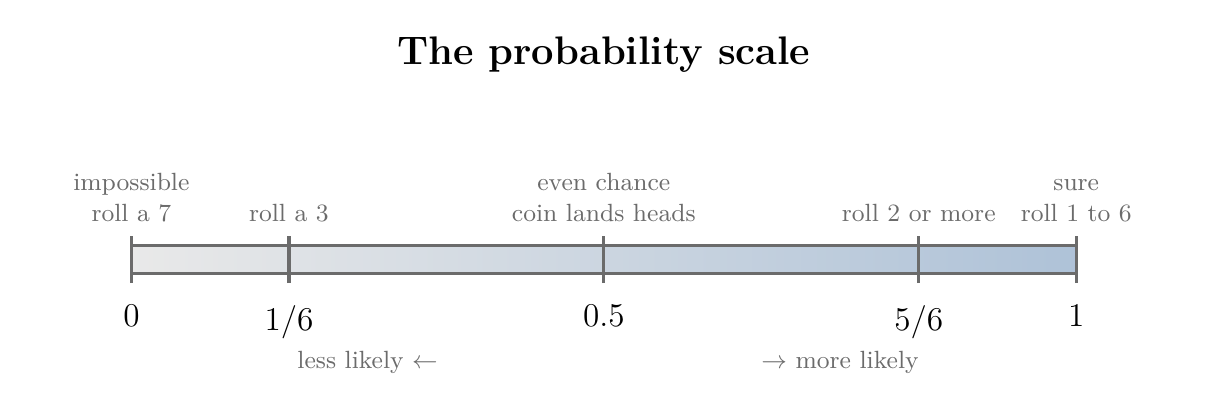
\begin{tikzpicture}[x=12cm, y=1cm]
  \node[title] at (0.5,2.6) {The probability scale};
  \shade[left color=cgrey!15, right color=cblue!45] (0,-0.18) rectangle (1,0.18);
  \draw[cgrey] (0,-0.18) rectangle (1,0.18);
  \foreach \p/\l in {0/0, 0.1667/{1/6}, 0.5/0.5, 0.8333/{5/6}, 1/1} {
    \draw[cgrey] (\p,-0.3) -- (\p,0.3);
    \node[below=4pt, font=\sffamily\large] at (\p,-0.3) {$\l$};
  }
  \node[note, above, text width=2.4cm] at (0,0.35) {impossible\\ roll a 7};
  \node[note, above, text width=2.4cm] at (0.1667,0.35) {roll a 3};
  \node[note, above, text width=2.4cm] at (0.5,0.35) {even chance\\ coin lands heads};
  \node[note, above, text width=2.4cm] at (0.8333,0.35) {roll 2 or more};
  \node[note, above, text width=2.4cm] at (1,0.35) {sure\\ roll 1 to 6};
  \node[note] at (0.25,-1.3) {less likely $\leftarrow$};
  \node[note] at (0.75,-1.3) {$\rightarrow$ more likely};
\end{tikzpicture}
\end{document}
